\subsection{Backend Tests}
The backend is a key part of the system as it handles all business logic and data storage in the system. Because 
the DBAccess class was made as a facade it made the most sense to us to do blackbox testing of it, as users of
the class would not have knowledge of its internal logic. Additionally, the backend is based heavily on the C\#
SQL library (\verb+System.Data.SqlClient+), and code branching happens mostly in this library. This argues against
using White Box testing.

The tests are done as automated unit tests to allow them
to be run everytime changes are made in the backend part of the system, thereby ensuring that everything is working as
intended.

To maximise the coverage in our backend tests we made a coverage table
(see Appendix \ref{app:dbtabs}) which describes what inputs should be tested.
Having the coverage table at hand when implementing the tests was great as it
ensured that we had the wanted coverage for all methods. It also allowed us to
split the implementation of the tests between us but still have the same
coverage level as the coverage table was done in collaboration. This did 
however lead to the unfortunate situation that the DBFilehandler file has not
been tested as we forgot to delegate its implementation.

For the tests described in the coverage tables we used the ClearDatabase method
to make the cleanup of the tests easier. This had the unfortunate side effect of
breaking the FileTest and UserTest, but as we deemed the testing of the DBAccess
class more important we chose to ignore this. 
\begin{figure}[hbt]
	\centering
	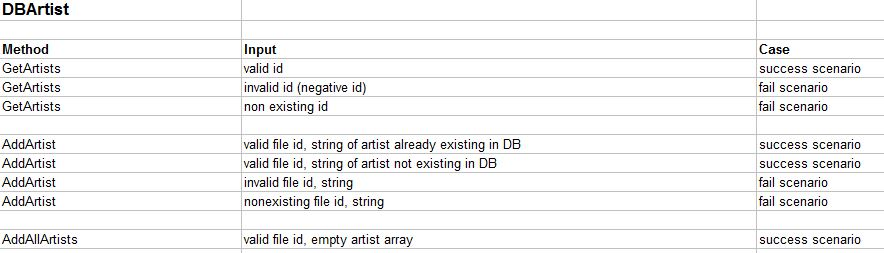
\includegraphics[scale=0.52]{./testing/coverage.jpg}
	\caption{Part of the coverage table for the backend tests}
	\label{fig:covtabs}
\end{figure}
